\section{Results}

% Detallad en este apartado los resultados obtenidos utilizando la metodología descrita en el apartado anterior.

\subsection{MSI-1's RRM1-orig docking model}

The first docking simulation performed with \texttt{LightDock} corresponded to the RRM1-orig RNA-motif complex. The simulation yielded several models out of which 10 were visualized, as shown in \textbf{Figure \ref{fig:allRRMorig}}:

\begin{figure}[htbp!]
    \centering
    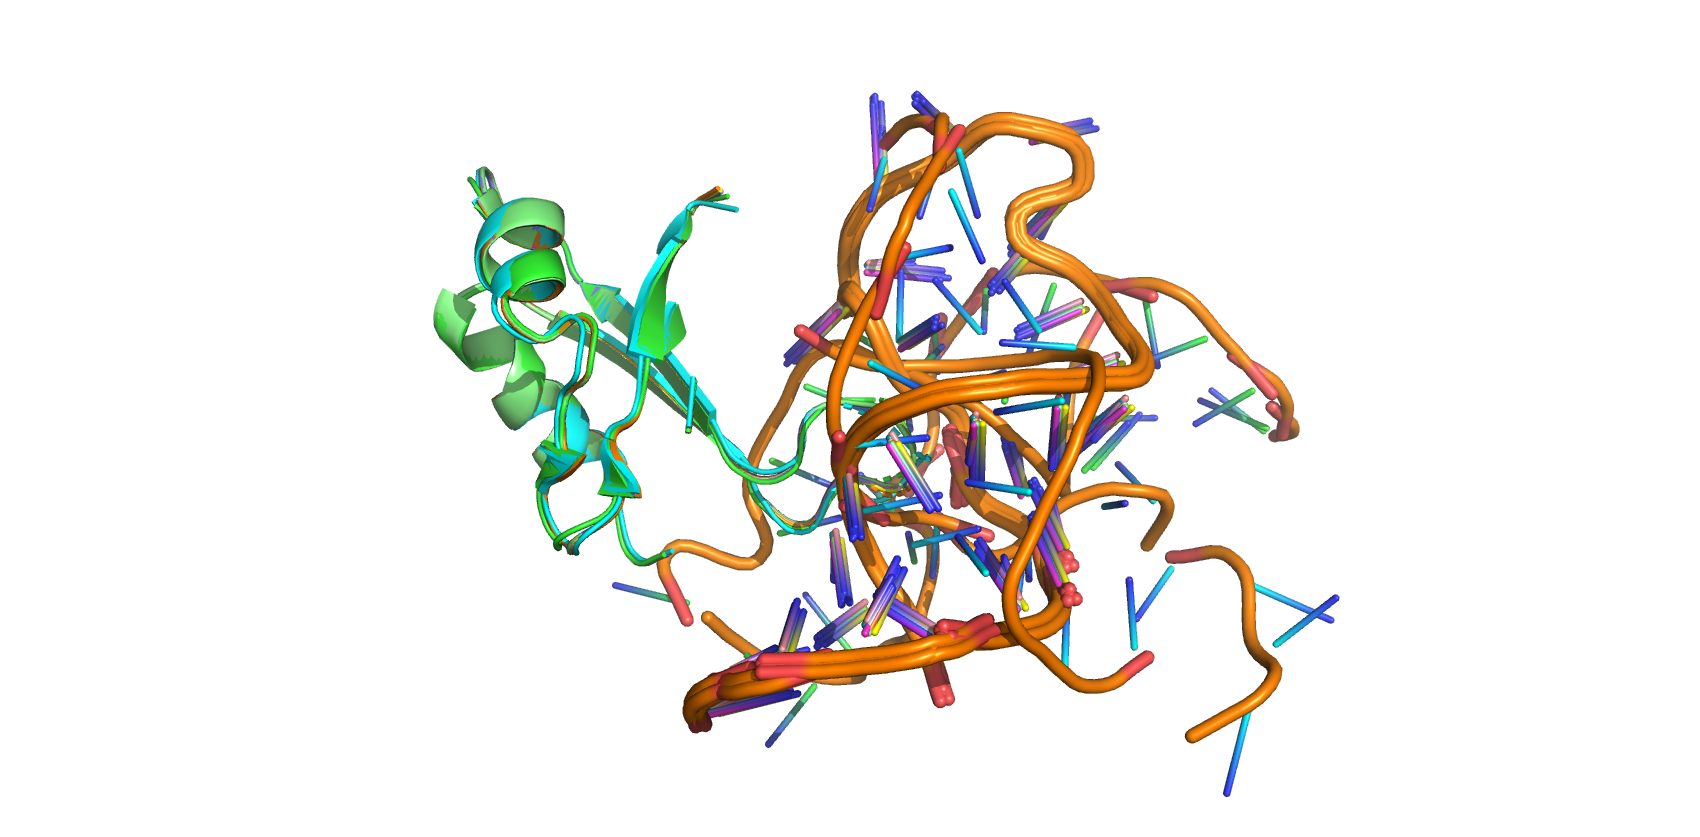
\includegraphics[width=0.82\linewidth]{assets/RMM1_orig_ALL.png}
    \caption[Top 10 scoring models for RRM1-orig RNA-motif complex.]{Top 10 scoring models for RRM1-orig RNA-motif complex. Visualized through \href{https://pymol.org/2/}{\texttt{Pymol}}.}
    \label{fig:allRRMorig}
\end{figure}

It is observed that there is no consensus among the top 10 scoring models, as it seems that the RNA-motifs adopts different conformations. To be more precise, in \textbf{Figure \ref{fig:allRRMorig}} there are 3 different RNA conformations. Their separate conformations are shown in \textbf{Figure \ref{fig:RRMorigSep}}:

\begin{figure}[htbp!]
\minipage{0.32\textwidth}
    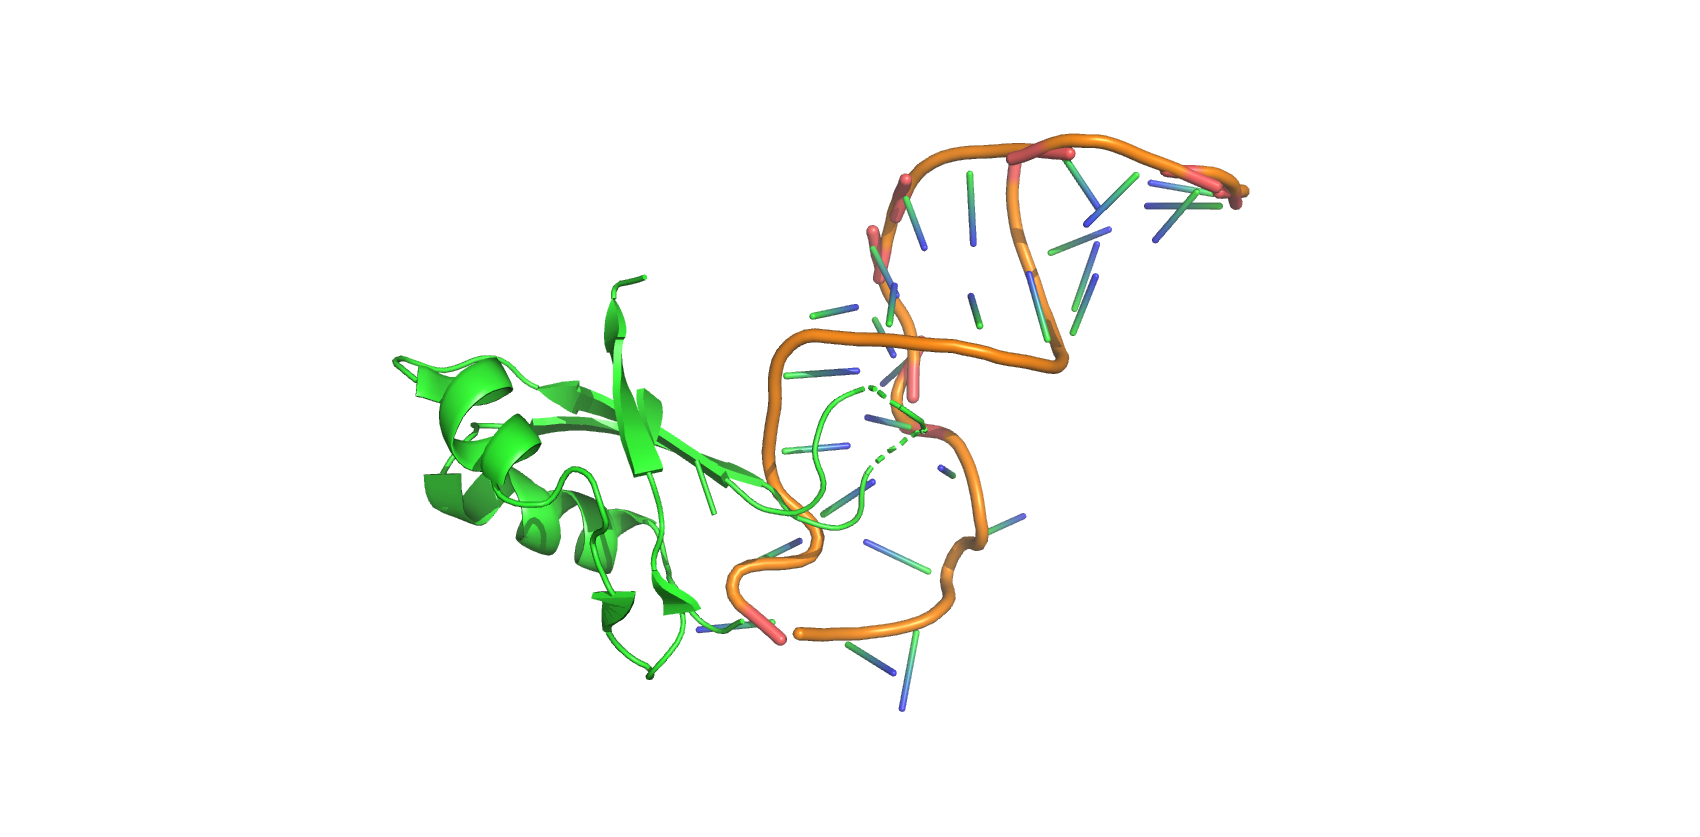
\includegraphics[trim={6.5cm 0 6.5cm 0},clip,width=\linewidth]{assets/RMM1_orig_top0.png}
\endminipage\hfill
\minipage{0.32\textwidth}
    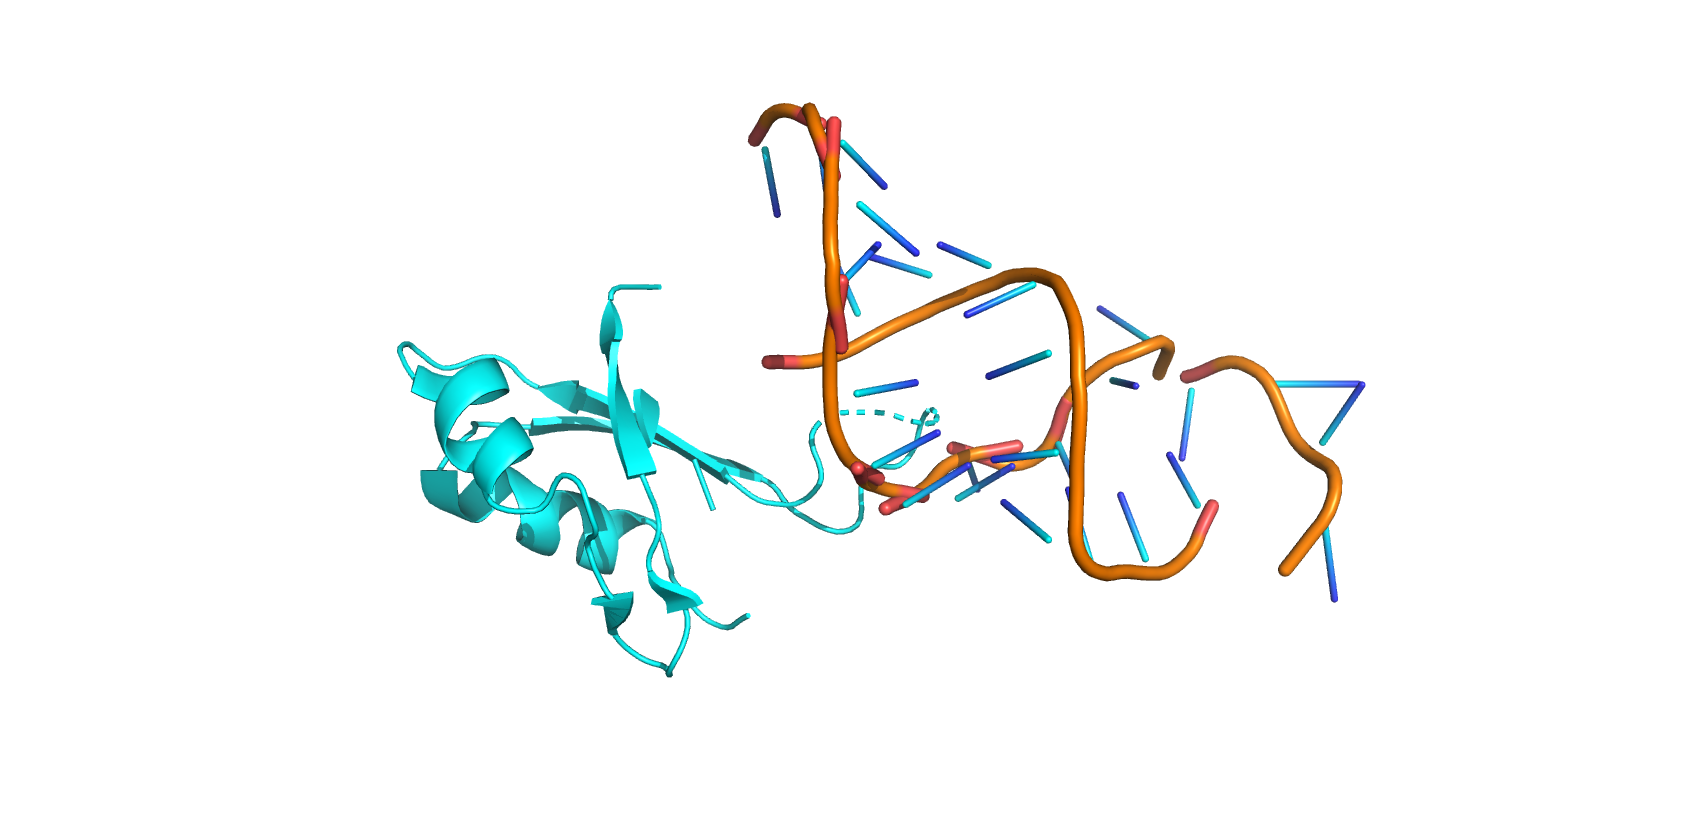
\includegraphics[trim={6.5cm 0 5.5cm 0},clip,width=\linewidth]{assets/RMM1_orig_top1.png}
\endminipage\hfill
\minipage{0.32\textwidth}
    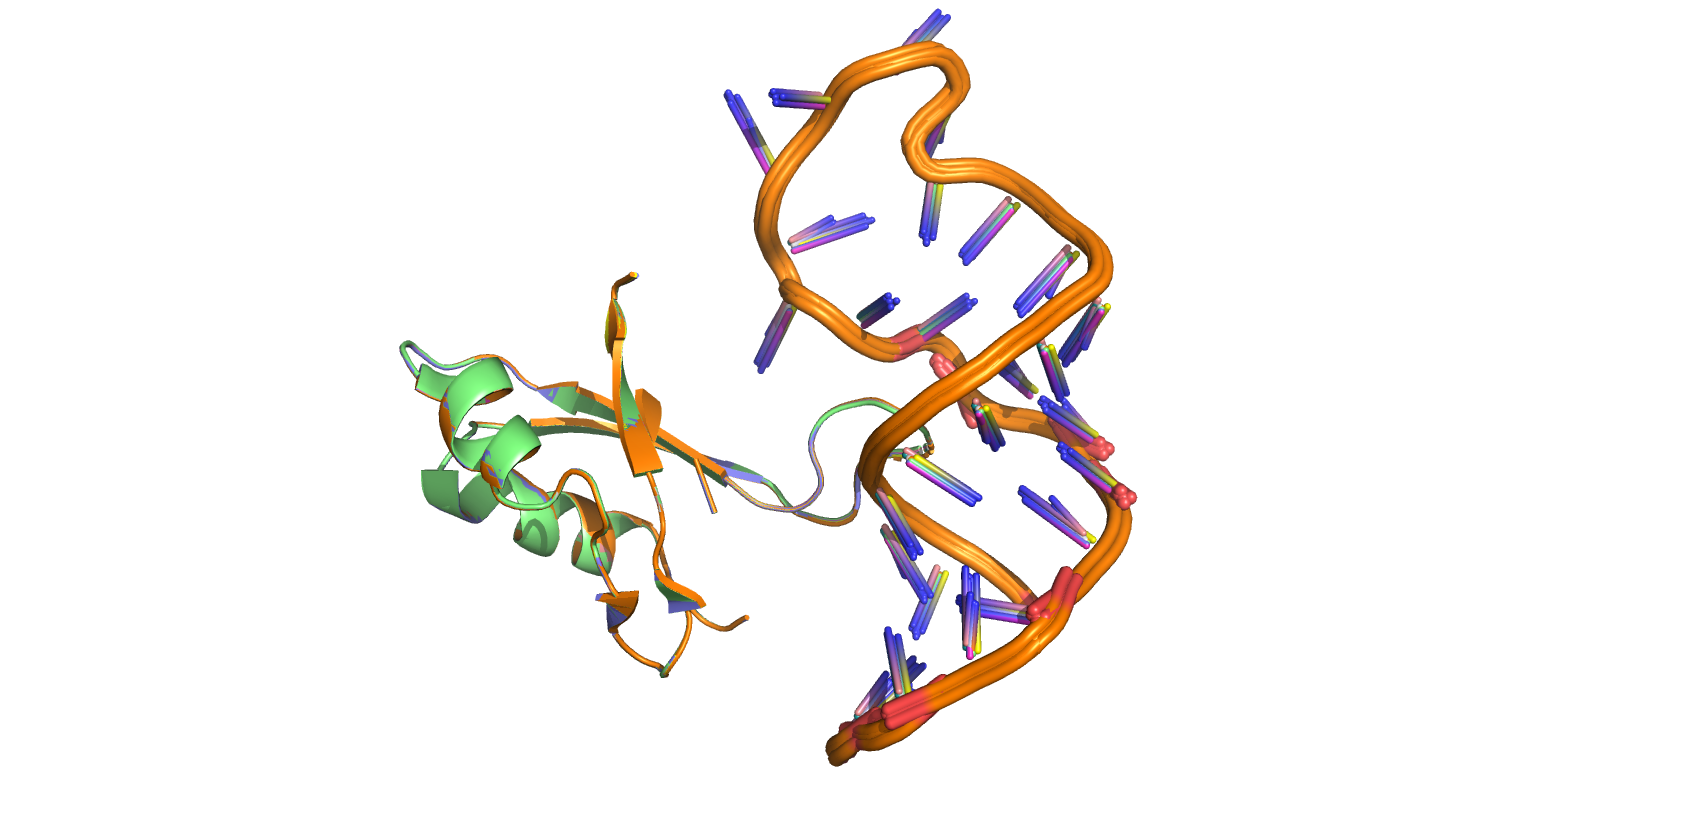
\includegraphics[trim={6.5cm 0 7cm 0},clip,width=\linewidth]{assets/RMM1_orig_2to8.png}
\endminipage
\caption[Top 10 scoring models for RRM1-orig RNA-motif complex grouped by RNA conformations.]{Top 10 scoring models for RRM1-orig RNA-motif complex grouped by RNA conformations. From left to right: best scoring model, second best scoring model and top 3 to 10 best scoring models. Visualized through \href{https://pymol.org/2/}{\texttt{Pymol}}.}
\label{fig:RRMorigSep}
\end{figure}


% Comentar lo que se ve

%         \item MSI-1 y el motivo de RNA original
%         \item MSI-1 y el motivo de RNA original (con estructura lineal)
%         \item MSI-1 y el mutante de RNA número 1
%         \item MSI-1 y el mutante de RNA número 2
%         \item MSI-1 y el mutante de RNA número 3
%         \item MSI-1 y el mutante de RNA número 4
%         \item MSI-1 y el mutante de RNA número 5
%     \end{itemize}

%     \item Selección de los 10 modelos de docking con mejor score de luciferina para cada una de las simulaciones mencionadas anteriormente.

%     \item Visualización de los modelos generados por \texttt{lightdock} mediante \texttt{pymol}.

%     Los resultados se encuentran en los siguientes anexos:
%     \begin{itemize}
%         \item\textbf{\nameref{anexo_E}}
%         \item\textbf{\nameref{anexo_F}}
%         \item \textbf{\nameref{anexo_G}}
%         \item \textbf{\nameref{anexo_H}}
%         \item \textbf{\nameref{anexo_I}}
%         \item \textbf{\nameref{anexo_J}}
%         \item \textbf{\nameref{anexo_K}}
%         \item \textbf{\nameref{anexo_L}}
%         \item \textbf{\nameref{anexo_M}}
%         \item \textbf{\nameref{anexo_N}}
%         \item \textbf{\nameref{anexo_O}}
%     \end{itemize}